% Ubah kalimat sesuai dengan judul dari bab ini
\chapter{PROFIL PERUSAHAAN}

% Ubah konten-konten berikut sesuai dengan yang ingin diisi pada bab ini

\section{Sejarah Departemen Teknik Komputer FTEIC - ITS}

Pada tanggal 10 Nopember 1957, Presiden Pertama RI, Dr.Ir. Soekarno meresmikan berdirinya Perguruan Tinggi Teknik Sepuluh Nopember di lapangan terbang Morokrembangan Surabaya.

Atas dasar PP No. 9 Tahun 1961, perguruan tinggi teknik tersebut dinegerikan dengan nama Institut Teknologi Sepuluh Nopember (ITS).

Pada saat berdirinya, Perguruan Tinggi Teknik Sepuluh Nopember hanya memiliki 2 Fakultas, yakni Fakultas Teknik Sipil (FTS) dan Fakultas Teknik Mesin (FTM). Setelah dinegerikan, ITS memiliki 3 Fakultas baru, yaitu Fakultas Teknik Elektro (FTE), Fakultas Teknik Kimia (FTK), dan Fakultas Teknik Perkapalan (FTP). Dengan SK Menteri PDK No. 72 Tahun 1965, ITS menambah 2 Fakultas lagi, yaitu Fakultas Teknik Arsitektur (FTA) dan Fakultas Ilmu Pasti dan Ilmu Alam (FIPIA).

Berdasarkan Keputusan Presiden RI No. 58 Tahun 1982 mengenai penataan kembali organisasi dan tata kerja ITS, Fakultas Teknik Elektro ITS berubah menjadi Jurusan Teknik Elektro. Dalam hal ini, Fakultas Teknik Mesin, Fakultas Teknik Elektro, Fakultas Teknik Kimia dan Jurusan Teknik Fisika FIPIA digabung menjadi Fakultas Teknologi Industri (FTI). Jurusan Teknik Multimedia dan Jaringan ITS (PSS TMJ – ITS) lahir dari salah satu bidang studi di Jurusan Teknik Elektro ITS (JTE – ITS) yaitu Bidang Studi Teknik Komputer dan Telematika (TKT). Sehubungan dengan hal tersebut diatas, PSS TMJ – ITS melakukan sharing resources dengan JTE ITS untuk saran dan prasarana serta SDM.

Jurusan Teknik Multimedia dan Jaringan FTI – ITS (PSS TMJ-ITS) berdiri dengan nomor SK Mentri Pendidikan Nasional No. 382/E/O/2012 tertanggal 9 Nopember 2012 yang ditanda tangani Menteri Pendidikan dan Kebudayaan.

Sedangkan Departemen Teknik Komputer ITS merupakan nama baru dari Jurusan Teknik Multimedia dan Jaringan ITS akibat adanya perubahan status ITS sebagai PTN-BH dan penyesuaian aturan penamaan program studi dalam Permendikbud No. 154 Tahun 2014. Permendikbud ini tidak mengubah status akreditasi A yang sudah didapatkan sebelumnya. Departemen Teknik Komputer ITS berada di Fakultas Teknologi Elektro ITS yang terdiri dari Departemen Teknik Elektro, Departemen Teknik Komputer,  Departemen Teknik Biomedik.

Kemudian pada Tahun 2014, sesuai SK rektor ITS PTNBH 2014, departemen berubah nama menjadi Departemen Teknik Komputer.

Periode 2017 – 2019, Berdirinya FTIK dan FTE. Fakultas Teknologi Elektro (FTE), Institut Teknologi Sepuluh Nopember (ITS) telah berjalan sejak januari tahun 2017 berdasarkan Peraturan Pemerintah No. 54 tahun 2015 dan Peraturan Rektor No. 10 tahun 2016. Didirikan Fakultas Teknologi Informasi dan Komunikasi dan Fakultas Teknologi Elektro . Fakultas Teknologi Informasi dan Komunikasi terdiri dari 3 departemen yaitu Departemen Informatika, Departemen Sistem Informasi, Departemen Teknologi Informasi. Fakultas Teknologi Elektro terdiri dari 3 departemen yaitu Departemen Teknik Elektro, Departemen Teknik Komputer, dan Departemen Teknik Biomedik.

Tahun 2020 berdiri Fakultas Teknologi Elektro dan Informatika Cerdas FT-EIC. Pada tahun 2020, Fakultas Teknologi Elektro dan Informatika Cerdas didirikan berdasarkan Peraturan Rektor No. 25 Tahun 2019 tentang OTK Institut Teknologi Sepuluh Nopember. FT-EIC terdiri dari 6 departemen yaitu Departemen Teknik Elektro, Departemen Teknik Komputer, Departemen Teknik Biomedik, Departemen Teknik Informatika, Departemen Sistem Informasi, dan Departemen Teknologi Informasi.

\section{Visi dan Misi}

\begin{enumerate}[nolistsep]

  \item \textbf{Visi Departemen Teknik komputer FTEIC - ITS}

	Menjadi departemen bereputasi internasional yang inovatif dan kreatif dalam bidang teknik komputer.

  \item \textbf{Misi Departemen Teknik komputer FTEIC - ITS}

  \begin{enumerate}[nolistsep]

    \item [1. ] Menyelenggarakan pendidikan yang berorientasi pada inovasi teknologi komputer dan implementasinya untuk masyarakat serta bereputasi internasional (pendidikan).

    \item [2. ] Menghasilkan lulusan yang profesional dan kreatif serta menguasai teknologi masa depan di bidang teknik komputer (pendidikan).

    \item [3. ] Mengembangkan penelitian yang terkini dan inovatif dalam bidang teknik komputer termasuk di dalamnya adalah pengembangan riset dalam Internet of Things, Data Science, Virtual Reality, Jaringan Komputer, Biomedical Engineering dan Big Data (penelitian).

    \item [4. ] Aktif berkontribusi dalam menyelesaikan permasalahan di masyarakat (abmas).

    \item [5. ] Aktif melakukan kerjasama internasional dalam bidang pendidikan dan penelitian (internasional).
  \end{enumerate}

\end{enumerate}

\section{Struktur Organisasi}

Struktur Organisasi dari Departemen Teknik Komputer FTEIC - ITS

% Contoh input gambar dengan format *.jpg
\begin{figure} [ht] \centering
  % Nama dari file gambar yang diinputkan
  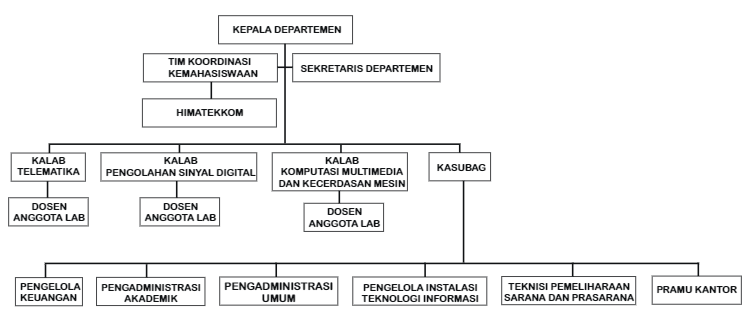
\includegraphics[scale=0.4]{gambar/organisasi.png}
  % Keterangan gambar yang diinputkan
  \caption{Struktur Organisasi DTK FTEIC - ITS}
  % \citep{DiscoverySpaceShuttle}
  % Label referensi dari gambar yang diinputkan
  \label{fig:Organisasi}
\end{figure}

% Contoh penggunaan referensi dari gambar yang diinputkan
Seperti yang bisa dilihat pada Gambar \ref{fig:Organisasi}, Dalam menjalankan kegiatan operasionalnya DTK-ITS telah membentuk struktur organisasi yang kompatibel dengan struktur organisasi ITS. Dalam pelaksanaan program DTK-ITS, Kepala Departemen dibantu oleh Sekretaris Departemen, Kepala staf non akademik (Kasubag TU) yang membantu dalam Sumber Daya Keuangan. Dalam melakukan kegiatan akademik dan operasional, Kasubag akan dibantu oleh para staf dengan fungsi staf masing-masing.
